\chapter{Plural marking of German noun insertions in bilingual sentences}\label{PL}

The study presented in this chapter\footnote{This chapter is based on an earlier publication, see \citep{hakimov}.} differs from the analyses reported in the previous chapters in that it explores mixing patterns in the expression of plural, i.e., at the level of the morphological word, whereas the studies in the previous chapters investigated code-mixing beyond the level of the morphological word. The focus on morphological processes has ramifications for the types of mixing patterns and the number of elements, or forms, competing for selection in bilingual speech production.

In Russian-German bilingual sentences in which Russian is the matrix language, embedded-language, i.e., German, nouns may either receive plural marking from Russian, or retain their German markers, for instance:

\ea (LV120224-11)\label{ex:6:1}\\
    \gll tam očen' xoroš-ie \textit{geschenk}-i. tam možno \textit{punkt}-y mnogo \textit{punkt}-ov sobra-t' na \textit{baby}-k-ax. na privivk-ax... na \textit{u} \textit{untersuchung-en}\\
        there very good-\textsc{nom.pl} present-\textsc{nom.pl.m} 
        there possible point-\textsc{nom.sg.m} many point-\textsc{nom.sg.m} collect-\textsc{inf} on baby-\textsc{dim}-\textsc{prep.pl} 
        on jab-\textsc{prep.sg.f} on check-up check-up\textsc{(f)-pl}\\
    \glt ‘They have very good presents. You can earn many bonus points for babies, for jabs, for check-ups.’
\z

\noindent This example contains several German nouns embedded in the Russian discourse. For now, let us focus on the nouns \textit{Geschenk} ‘present’ and \textit{Untersuchung} ‘check-up’. The former noun receives the Russian inflectional suffix \textit{-i} cumulatively expressing several categories including the plural, whereas the latter noun is inserted together with its German plural marker \textit{-en}.\footnote{The analysis of the noun \textit{Punkt} ‘(bonus) point’ is less straightforward. I am inclined to analyse it as a German insertion because the Russian word \textit{punkt} does not refer to a bonus point, which is commonly expressed as \textit{ball}. The speaker, who grew up in Germany, is likely to be unfamiliar with the Russian expression since the system of bonus points is a relatively new phenomenon in Russia. Yet, an orthodox analysis would have to conclude that this item is not a German insertion. The next noun is the German acronym \textit{U}, utilised by a specific German health insurance company for \textit{Untersuchung} ‘check-up’. The speaker handles it as a Russian indeclinable noun, which is in line with the Russian grammar. Finally, the German noun \textit{Baby} receives both an inflectional and a derivational, namely, diminutive suffix (for more details, see \sectref{morph-restr}).} Again a distinction is made between mixed constituents (e.g., \textit{geschenki}) and embedded-language islands (e.g., \textit{untersuchungen}). Crucially, the speaker might have handled these words differently, producing the embedded-language island \textit{geschenke} and the mixed constituent \textit{untersuchungax}. It is the choice between these two patterns of plural marking, which is the object of study in this chapter. Unlike the embedded-language islands analysed in the previous chapters, the islands examined here lack syntactic independence and are labelled as internal embedded-language islands \citep[][149--150]{myers-scotton-contact-2002}\footnote{The problem with considering embedded-language plurals as syntactically independent was raised by \citet[][36--37]{boumans-syntax-1998}. I agree that this view is difficult to maintain for language constellations in which at least one of the languages relies on affixes fusing the number and the morphological case, such as Russian. Yet, I will keep this term in order to highlight the difference between embedded-language islands representing co-occurrences of words and those representing morpheme co-occurrences.}. Embedded-language plurals have often been discussed in the literature (see \citealt{backus-two-1996, backus-evidence-1999, backus-units-2003, boumans-syntax-1998, muhamedowa-untersuchung-2006,myers-scotton-duelling-1993, myers-scotton-contact-2002}), but the proposed explanations for their emergence are still a matter of controversy. The question I address in this chapter is whether variation in patterns of plural marking of code-mixed nouns can be effectively predicted by a combination of structural and usage-based factors.

The first hypothesis of this study is that the frequency distribution of singular and plural forms in the embedded language, German, will influence patterns of plural marking of German nouns in Russian sentences. Words that are often used in their plural forms in one language are inserted as plurals into another language \citep{backus-two-1996, backus-evidence-1999, backus-units-2003}. Highly entrenched German plurals will thus retain German plural markers in Russian sentences. Another consequence of the frequency distribution of singular and plural forms in the embedded language is that nouns frequent in the singular in German will receive their plural marking from Russian, the matrix language. As a matrix language, Russian restricts the possibilities for accommodation of German noun insertions on the morphophonological level. The Russian nominal system favours stems featuring consonants in the final position. Therefore, the second hypothesis is that German noun stems exhibiting vowels stem-finally will retain the German plural marker. That is, the phonemic shape of German nouns is a factor determining the choice of language for marking the plural on inserted stems. Another motivation behind the observed variation is a mismatch between the nominal systems of German and Russian: the Russian system exhibits a lesser degree of syncretism and contains more morphological cases than German. The final hypothesis is therefore that an insertion will receive a Russian plural affix if the slot of the insertion requires a non-core case. This is of particular interest in a situation of contact between Russian and German, two fusional languages, as previous research on variation in plural marking of noun insertions has thus far only involved pairs of agglutinative and analytical languages.

This chapter is organised as follows: Section 1 presents a survey of patterns of plural marking on code-mixed nouns by drawing on instances observed in corpora of bilingual speech involving various language pairs. Section 2 reports the state of the art of code-mixing research concerned with explaining the distribution of these patterns in mixed sentences. Section 3 then offers an overview of the systems of plural marking in Russian and German. Section 4 is concerned with the analysis of the factors determining the studied variation: these include the frequencies of the singular and plural forms of the inserted lexical items as distributed in the embedded language, phonemic shape of the German noun insertions, including the segment featured stem-finally, and the morphosyntactic context in which the nouns appear, i.e., the morphological case required by the slot in which they are to be inserted. Each of these factors is a tendency rather than an absolute rule, therefore they are evaluated statistically in Section 5, which describes the statistical model testing the interplay of factors when predicting the use of the examined patterns. Section 6 summarises and discusses the results.

\section{Typology of marking plural on code-mixed nouns}

Code-mixed nouns can receive plural marking in three different ways: the first possibility  results from the morphological processes of the matrix language, as in (\ref{ex:6:2a}); the second possibility to mark the plural on code-mixed nouns is to retain the plural marker used with the word in the embedded language, i.e, the language of the inserted stem, as in (\ref{ex:6:2b}); the final option is double plural marking, which refers to the case when the noun receives two plural markers: one from the embedded language and the other from the matrix language, as in (\ref{ex:6:2c}).

\ea 
\ea
	\textsubscript{A}[ \textsubscript{B}[ N \textsubscript{B}]-\textsc{pl} \textsubscript{A}]\label{ex:6:2a}
\ex	{\textsubscript{A}[ \textsubscript{B}[ N-\textsc{pl} \textsubscript{B}] \textsubscript{A}]}\label{ex:6:2b}
\ex	{\textsubscript{A}[ \textsubscript{B}[ N-\textsc{pl} \textsubscript{B}]-\textsc{pl}}\textsubscript{A}]\label{ex:6:2c}
\z
\z

\subsection{Type 1: A morphological process of the matrix language}

Marking the plural by the morphological process of the matrix language is especially frequent in situations in which the matrix language is an agglutinative language. In (\ref{ex:6:3}), the Dutch noun \textit{activiteit} `activity', embedded into a Turkish clause, is used with the Turkish plural suffix -\textit{ler}-, and in (\ref{ex:6:4}), the English noun \textit{rule} acquires the Finnish stem formant -\textit{i} and the plural marker -\textit{t}. 

\ea
\label{ex:6:3}
Turkish-Dutch \citep[150]{backus-two-1996}\\
\gll \textit{activiteit}-ler-i {yapacağız} {dedik}\\
	activity-\textsc{pl-acc} do:\textsc{fut;1pl} said:\textsc{1pl}\\
\glt `we said we were going to activities'
\ex
\label{ex:6:4}
Finnish-English \citep[60]{halmari-government-1997}\\
\gll {joo} {missä} {kummassa} {ne} \textit{rule}-i-t {on}?\\
	yeah where ever \textsc{3pl} {\phantom{mm}}-\textsc{sf-pl} are\\
\glt `Yeah, where on earth are those rules?'
\z

\noindent The high frequency of this kind of insertion in language pairs with an agglutinative language as the matrix language, and its rarity in pairs of languages with fully fusional Arabic (\citealt[180]{boumans-syntax-1998}; \citealt[189]{nortier90}) and moderately fusional French and Dutch as the matrix language \citep{treffers-daller-mixing-1994} led Muysken to hypothesise that fusional languages are resistant to this pattern (\citeyear[77]{muysken-bilingual-2000}). However, from as early as \citet[265--266]{hasselmo72} there is documented evidence in the literature against this claim (see \citealt[174]{budzhak-jones98}, for Ukrainian-English; \citealt[73]{hlavac-second-generation-2003}, for Croatian-English; \citealt[180]{stenson-1990}, for Irish-English; \citealt[352]{szabo-language-2010}, for German-Hungarian). In line with this evidence are the following examples of embedded-language nouns in Russian sentences:

\ea
\label{ex:6:5}
Russian-English \citep[173]{benson}\\
\gll ves' \textit{place} by-l zaparkova-n \textit{car}-ami\\
	whole place$[$\textsc{nom.sg}$]$ be-\textsc{pst}$[$\textsc{sg.m}$]$ park-\textsc{part$[$sg.m$]$} \phantom{mn}-\textsc{instr.pl}\\
\glt `The whole place was parked full of cars.'
\ex
\label{ex:6:6}
Russian-Hebrew \citep[48]{naiditch08}\\
\gll {kogda} {u} {vas} {nač-n-ut-sja} \textit{bagrut}-y?\\
	when with \textsc{2gen.pl} begin-\textsc{perf-3pl-refl} exam-\textsc{nom.pl}\\
\glt `When will your exams begin?'
\z

\noindent The nouns \textit{car} in (\ref{ex:6:5}) and \textit{bagrut} `exam' in (\ref{ex:6:6}) take Russian inflectional affixes expressing the plural and a morphological case, which is also a typical pattern in the Russian-German code-mixing data analysed below.

\subsection{Type 2: A morphological process of the embedded language}

As mentioned above, another possibility to express the plural on noun insertions in bilingual sentences is to resort to a process employed by the embedded language so that an internal embedded-language island occurs. In (\ref{ex:6:7}), the noun \textit{window} is inserted together with its English plural marker -\textit{s}; similarly in (\ref{ex:6:8}), the plural form \textit{dvarim} `things' of the Hebrew noun \textit{davar} is embedded in the Russian clause.

\ea
\label{ex:6:7}
Russian-English \citep[173]{benson}\\
\gll {ona} {poš-l-a} \textit{clean}-ova-t' \textit{window-s}\\
	\textsc{3sg.f} go-\textsc{pst-sg.fs} \phantom{mmn}-\textsc{sf-inf} \phantom{mmmm}-\textsc{pl}\\
\glt `She went to clean windows.'
\ex
\label{ex:6:8}
Russian-Hebrew \citep[48]{naiditch08}\\
\gll {est'} {neskol'ko} \textit{dvar-im} {kotor-ye} {my} {dolžn-y} {zna-t'}\\
	be.\textsc{prs} several \textsc{pl}\textbackslash thing-\textsc{pl} which-\textsc{acc.pl} \textsc{1pl} obliged-\textsc{1pl} know-\textsc{inf}\\
\glt `There are several things we have to know.'
\z

\noindent Both plurals in (\ref{ex:6:7}) and in (\ref{ex:6:8}) lack case marking, which is required in Russian, and thus count as internal embedded-language islands. The Russian sentence in (\ref{ex:6:9}) contains the Estonian form \textit{vaimusid} ‘ghosts’, which is inflected for the partitive case. This is obviously possible owing to a functional similarity in this specific context between the Estonian partitive and the Russian genitive, required by the verb \textit{bojus’} ‘am afraid’.

\ea
\label{ex:6:9}
Russian-Estonian (\citealt[117]{muerkhein}, quoted from \citealt[437]{verschik04})\\
\gll {ja} {boj-u-s'} \textit{vaim-u-sid}\\
	\textsc{1sg} fear-\textsc{1sg-refl} ghost-\textsc{sf-partitive.pl}\\
\glt `I am afraid of ghosts.'
\z

Some agglutinative languages, such as Tamil and Kazakh \citep[67]{muhamedowa-untersuchung-2006}, have been reported to combine  embedded-language plural markers with matrix language case markers, as in (\ref{ex:6:10}). This is indicative of the gradience of the morphosyntactic integration of noun insertions.

\ea
\label{ex:6:10}
Tamil-English \citep[81]{sankoff-et-al-1990}\\
\gll only {kalaimagaLLataan} \textit{movie-s}-e {patti} {peece} {ille}\\
	only proper.name.\textsc{loc}.only movie-\textsc{pl-acc} about talk \textsc{neg}\\
\glt `Only in KalaimagaL there is no talk about the movies.'
\z

\subsection{Type 3: Double plural marking}

\noindent Double plural marking is probably the most frequently described case of double morphology documented in the literature and has therefore attracted the most scholarly interest (\citealt[96]{backus-patterns-1992}, \citeyear[151]{backus-two-1996}, \citeyear[98--99]{backus-evidence-1999}; \citealt[90--91]{boumans-syntax-1998}; \citealt[152--156]{muhamedowa-untersuchung-2006}; \citealt[132--135]{myers-scotton-duelling-1993}, \citealt{myers-scotton-matching-1995}). For example:

\ea
\label{ex:6:11}
Kazakh-Russian \citep[152]{muhamedowa-untersuchung-2006}\\
\gll {sonday} {ülken} \textit{zvanij-a}-lar-ï {bar}\\
	such big title-\textsc{pl.nom-pl-pos3sg} \textsc{exist.3sg}\\
\glt `He has many titles.'
\z

\noindent Here the Russian plural noun \textit{zvanija} `titles' additionally receives the Kazakh plural marker \textit{-lar-}. Another example comes from Moluccan Malay-Dutch code-mixing in the Netherlands and showcases the use of reduplication as a productive process of plural marking in Moluccan Malay \citep[50--56]{voigt94}:

\ea
\label{ex:6:12}
Moluccan Malay-Dutch \citep[52]{voigt94}\\
\gll {kalau} {minum} {terus} {ada} {di punya} \textit{pitje-s-pitje-s}-nya\\
	if drink continue exist \textsc{det} seed-\textsc{pl}-seed-\textsc{pl-det}\\
\glt `If I continue drinking there’ll be seeds.'
\z

\section{Previous explanations}

Prior studies have predominantly focused on double plural marking in mixed nouns, and double morphology in general, since the latter was considered an exceptional case in the early version of Myers-Scotton's \citeyear{myers-scotton-duelling-1993} influential Matrix Language Frame (MLF) model. The proponents of the MLF model attributed double morphology to erroneous access in production (\citealt[132--136]{myers-scotton-duelling-1993}; \citealt[1000]{myers-scotton-matching-1995}). Although \citet[134]{myers-scotton-duelling-1993} suggests possible scenarios for double morphology, it is not clear what factors determine its occurrence in bilingual corpora.

A structural explanation of the phenomenon was suggested by \citet[][91]{boumans-syntax-1998}, who considers a mismatch in the morphological marking processes to be a crucial factor determining the emergence of double morphology. According to Boumans, ``[t]he likelihood of double marking appears to increase when each language marks the same feature in a different manner, for instance, by means of prefixes and suffixes'' (ibid.). This approach sheds light on a number of cases of double morphology found in bilingual corpora, including, for instance, the Moluccan Malay-Dutch example (\ref{ex:6:12}). The morphological processes of plural marking mismatch in this case because Malay uses reduplication whilst Dutch employs suffixes. The dissimilarity leads to the emergence of a form with the plural marked twice. Boumans' proposal has been widely echoed in the literature. Indeed, it not only holds for double plurals, but also for other cases of double morphology (see \citealt[91]{myers-scotton-contact-2002}, for double marking of determiners and infinitives; \citealt[104]{muysken-bilingual-2000} and \citealt[152--156]{muhamedowa-untersuchung-2006}, for doubled adpositions; \citealt[346--352]{szabo-language-2010}, for doubled adpositions and determiners). \citet[150]{myers-scotton-contact-2002} extends this principle to the case of plural marking on inserted nouns by the embedded language. It can, for example, aptly account for the emergence of the internal embedded-language island in (\ref{ex:6:8}). Its emergence may be attributed to differences in the morphological processes involved in plural marking: while Hebrew relies on both stem change and suffixation, Russian draws only on inflectional suffixes.

This factor, however, has a restricted explanatory power for it cannot account for the use of double morphology in two cases. First, it is silent on the appearance of embedded-language islands in bilingual speech involving languages which use similar morphological processes for marking a particular feature, such as Kazakh and Russian (cf. example \ref{ex:6:11}). Second, even when the processes for marking plural do diverge, embedded-language markers may alternate with matrix language markers, as in (\ref{ex:6:13}):

\ea
\label{ex:6:13}
English-Hebrew \citep[70]{olshtain-blum}\\
\begin{tabularx}{\linewidth}{@{}lQ@{}} 
	Mother: & What do I have to do when I go to your \textit{gan} (nursery.school)?\\
	Son (15): & Wait, they are on strike, the \textit{gan-im} (nursery.school\textsc{-pl})? \\
	Mother: & No, the \textit{ozrot} (\textsc{pl}\textbackslash assistant) are on strike. In order not to close down the \textit{gan} the mothers are taking \textit{tor-ot} (turn-\textsc{pl}) to help the \textit{ganenet}-s (nursery.teacher-\textsc{pl}). The assistants to the  \textit{ganenet}-s (nursery.teacher-\textsc{pl}). They're young women who have taken a year's course to be an \textit{ozeret} (assistant) for \textit{gan-im} (nursery.school-\textsc{pl}).\\ 
    Son (15): & So why are they going on strike and not the \textit{gananot} (\textsc{pl}\textbackslash nursery.teacher)? \\
\end{tabularx}
\z

\noindent This example demonstrates high variability of plural marking within a short piece of conversation. Hebrew morphology is retained in most of the plural forms: \textit{ganim} `nursery schools', \textit{ozrot} `assistants', \textit{torot} `turns' and \textit{gananot} `nursery teachers'. Of these plurals, the forms \textit{ozrot} and \textit{gananot} can be explained by a mismatch in the morphological processes because they express the plural by using stem change, and not suffixation as English nouns. Nevertheless, on another occurrence the noun \textit{ganenet} `nursery teacher' receives the English plural marker \textit{-s}.

In discussing the same phenomenon, \citet[151]{backus-two-1996} posits an alternative proposal. Within a Cognitive Linguistics framework, he provides a usage-based explanation of double marking. Emphasising the role of entrenchment of certain plural forms, he observes that some nouns occur in their plural form more often than in their singular form. The high degree of entrenchment of these plural forms leads to a facilitation of their activation in production, and is attributed to a mismatch in the frequency distribution of the plural and singular forms of nouns. In his later work, \citet[98]{backus-evidence-1999} elaborates this idea further : ``[\dots{} embedded-language plurals] are established lexical units for the speakers who use them. This means they are chunks [\dots{}]: they are lexical units that consist of more than one morpheme.'' This assumption is based on the idea that the strength of cognitive representations at various linguistic levels is a function of usage frequency, and it is thus in line with usage-based linguistic theory \citep{bybee-morphology-1985,bybee-repetition-2006,bybee-book-2010}. A rich memory for language \citep{langacker-foundations-1987,langacker00,tomasello-constructing-2003,bybee-book-2010} allows for both plural and singular forms of same nouns to exist independently in the lexicon. (More details, including the findings on the processing of singulars and plurals, are reported in \sectref{processing}.) Although Backus's reasoning is highly  plausible, it cannot be viewed as a single principle determining the emergence of embedded-language plurals. If this were the case, any embedded-language noun that appeared with an embedded-language plural marker would be granted the status of a lexical unit. When modelling the probability of activating a plural form in production, we need to consider the competition between the representations of plural and singular forms of the inserted lexemes. \citet[][97]{baayen-dijkstra-schreuder} describe this competition in terms of distribution dominance and distinguish between singular-dominant and plural-dominant nouns: “Either the singulars were much more frequent than their plurals (singular-dominant) or the plurals had a much higher surface frequency than their singulars (plural-dominant pairs).”

As to other factors, phonotactic restrictions and morphophonological regularities have been largely neglected in the literature as possible motivations for the use of  plural marking patterns. However, as will be shown below, they are among important requirements imposed by the matrix language on items that are to be inserted in the structure it frames.

In sum, the appearance of embedded-language plurals as internal embedded-language islands, or as parts of double-marked constituents can be attributed either to a mismatch in the processes of plural marking, or singular-plural distribution dominance, i.e., an asymmetry in the token frequency of a lexical item’s singular and plural. Some other factors such as morphophonology have not yet been considered pertinent thus far. A limitation that pervades all the approaches to double morphology discussed is their sole reliance on individual factors and therefore a tendency to overlook the multi-factorial nature of the phenomenon. In order to account for the variation in the data, we need to analyse the possible driving forces behind it systematically and in their interaction.

\section{Plural marking in Russian and German}

Russian-German code-mixing provides a good testing ground for the interaction of factors that contribute to variable patterns of plural marking because they fusional languages. Both inflect nouns for number, gender and case, but demonstrate varying degrees of syncretism and systematicity in the encoding of these grammatical categories.

\subsection{Russian}

Russian noun declension fuses case, number, and gender marking. The system is stem-based and synthetic, and can be best described by stipulating declensional classes. However, there is no consensus in the literature regarding the number of the declensional classes and the determinants for distinguishing them (cf. \citealt{corbett91,corbett03}). In this paper I adopt Zaliznjak's \citeyear{zaliznjak02}, \citeyear{zaliznjak09} approach to the Russian nominal inflection. The following declensional classes are relevant for the presentation of the data below: the “masculine”, the “feminine”, and the zero-marked class. Based on the gender and phonological type of the stem, three principal classes are traditionally differentiated, each being prototypical for the respective gender: the masculine, the feminine, and the neuter. The three classes are presented in \ref{tab:6:1}. Of these classes, the “masculine” and “feminine” classes are the most productive ones (\citealt[218]{zaliznjak02}; \citealt[148]{timberlake04}). It is thus not surprising that they play a crucial role in the integration of the other-language noun stems in Russian sentences in bilingual speech. This tendency has been reported for Russian-Hebrew code-mixing \citep{naiditch08} and is observed in my Russian-German data. Crucially, the distinctions between the declensional classes in the plural, when compared to those in the singular, are minimal: each morphological case has one inflection per class except for the genitive and the nominative, whose forms coincide with those of the accusative.

\begin{table}
	\fittable{\begin{tabular}{ll *{3}{>{\centering\arraybackslash}p{\widthof{-y (-i)}}} *{3}{>{\centering\arraybackslash}p{\widthof{-ov (-ej)}}}}
	    \lsptoprule
		\multicolumn{2}{c}{} & \multicolumn{3}{c}{singular} & \multicolumn{3}{c}{plural}\\\cmidrule(lr){3-5}\cmidrule(lr){6-8}
		\multicolumn{2}{c}{} & m & n & f & m & n & f\\\midrule
		\multicolumn{2}{l}{nominative} & ∅ & -o & -a & -y (-i) & -a & -y (-i)\\
		\multicolumn{2}{l}{genitive} & \multicolumn{2}{c}{-a} & -y (-i) & -ov (-ej) & \multicolumn{2}{c}{∅}\\
		\multicolumn{2}{l}{dative} & \multicolumn{2}{c}{-u} & -e & \multicolumn{3}{c}{-am}\\
		accusative & inanimate & ∅ & -o & -u & -y (-i) & -a & -y (-i)\\
		accusative& animate & -a & -o & -u & -ov (-ej) & \multicolumn{2}{c}{∅}\\
		\multicolumn{2}{l}{instrumental} & \multicolumn{2}{c}{-om} & -oj & \multicolumn{3}{c}{-ami}\\
		\multicolumn{2}{l}{prepositional} & \multicolumn{3}{c}{-e} & \multicolumn{3}{c}{-ax}\\
		\lspbottomrule
	\end{tabular}}
	\caption{Inflections of the Russian nominal declension (adapted from \citealt[26]{zaliznjak09}).\label{tab:6:1}}
\end{table}

The last relevant class relies on zero marking and is restricted to a group of loan words ending in vowels, except unstressed \textit{-a} preceded by a consonant \citep[148--149]{timberlake04}. This class includes nouns such as \textit{xudi} ‘hoodie’, \textit{boa} `feather boa', \textit{kafe} `cafè', \textit{kenguru} `kangaroo', \textit{kino} `cinema'. None of the nominal grammatical categories is marked overtly on the nouns of this class; compare \textit{ljubimoe kafe} `a favorite cafè' versus \textit{raznye kafe} `different cafès'.

Russian employs the genitive singular to express plurality when nouns follow the cardinal numerals two, three, and four, for example: \textit{dv-a dom-a} `two-\textsc{m} house-\textsc{gen.sg.m}' and \textit{dv-e knig-i} `two-\textsc{f} book-\textsc{gen.sg.f}'. If we assume conceptual plurality, the instances of German noun insertions \textit{dv-a mensch-a} `two-\textsc{m} person-\textsc{gen.sg.m}' and \textit{dv-e flasch-i} `two-\textsc{f} bottle-\textsc{gen.sg.f}' should be considered as a case of plural marking.

\subsection{German}\label{german}

Like Russian, German noun inflection fuses case, number, and gender marking. Furthermore, the nominal system is also traditionally analysed in terms of declensional classes (\citealt[158]{eisenberg06}; \citetitle[229]{duden-2009}). Because the plural demonstrates a high degree of syncretism, some scholars handle the patterns of plural marking and the patterns of the nominal inflection in the singular separately, given that overt case marking is the exception in the paradigm \citep{flaemig, helbig-buscha,hentschel-weydt}. In the plural, the only case opposition, characteristic of most patterns of plural marking, is between the dative, which is marked by the suffix -\textit{(e)n}, and the non-dative. Interestingly, German noun insertions in my data set never carry the exponent of the dative in the plural. In other words, these German plurals do not exhibit German case morphology.

German employs four mechanisms of plural marking \citep[480]{flaemig}: (i) zero marking (\textit{Schüler} `pupil[\textsc{sg}])' -- \textit{Schüler} `pupil[\textsc{pl}]'), (ii) the use of umlaut, or vowel alternation (\textit{Garten} `garden[\textsc{sg}]' -- \textit{Gärten} `\textsc{pl}\textbackslash{}garden'), (iii) suffixation (\textit{Arm} `arm[\textsc{sg}]' -- \textit{Arm-e} `arm-\textsc{pl}'), (iv) a combination of umlaut and a plural suffix (\textit{Buch} `book[\textsc{sg}]' -- \textit{Büch-er} `\textsc{pl}\textbackslash{} book-\textsc{pl}'). The patterns of German plural marking, drawing on these mechanisms, are given in \tabref{tab:6:2}.

\begin{table}
\begin{tabular}{c lccl}
 \lsptoprule
	Pattern no. & Example of singular & \multicolumn{2}{c}{Pattern} & Example of plural \\\cmidrule(lr){3-4}
	& & Suffix & Umlaut & \\\midrule
	1 & \textit{Lehrer} `teacher'	& -∅	& \textminus & \textit{Lehrer}\\
	2 & \textit{Kloster} `cloister' & -∅	& + & \textit{Klöster}\\
	3 & \textit{Tag} `day' & -e	& \textminus & \textit{Tage}\\
	4 & \textit{Kopf} `head' & -e	& + & \textit{Köpfe}\\
	5 & \textit{Kind} `child' & -er	& \textminus & \textit{Kinder}\\
	6 & \textit{Mann} `man' & -er	& + & \textit{Männer}\\
	7 & \textit{Name(n)} `name' & -n	& \textminus & \textit{Namen}\\
	8 & \textit{Mensch(en)} `person' & -(e)n	& \textminus & \textit{Menschen}\\
	9 & \textit{Auto} `car' & -s	& \textminus & \textit{Autos}\\
	\lspbottomrule
	\end{tabular}
	\caption{Patterns of German plural marking (adapted from \citealt[480]{flaemig}).\label{tab:6:2}}
\end{table}

\section{Patterns of plural marking on code-mixed German nouns in the bilingual corpus}

A total of 153 German noun insertions in Russian sentences were identified in my corpus of Russian-German bilingual speech as marked for the plural. The German nominalised adjectives \textit{Mehrsprachige} `multilinguals', \textit{Russlanddeutsche} `Russian Germans' and \textit{Verwandte} `relatives' were not counted as nouns because they decline like adjectives and do not have stable plural forms.

Russian plural markers are found on 72 insertions. Together with the plural number, these forms also express all possible morphological cases. In (\ref{ex:6:14}), for instance, the German noun \textit{Augenarzt} `ophthalmologist' is used with the Russian inflection of the genitive plural.

\ea
\label{ex:6:14}
(LA050310)\\
\gll {malo} \textit{augenarzt}{-ov}\\
	few ophthalmologist-\textsc{gen.pl}\\
\glt `There are few ophthalmologists.'
\z

\noindent Of the German noun insertions found in the corpus, 69 appear with German plural markers, as in \REF{ex:6:15}.

\ea
\label{ex:6:15}
(LG050311)\\
\gll {čë} {na} {nej} {za} \textit{klamotte-n} {ode-t-y}\\
	what on \textsc{3prep.sg} for rag-\textsc{pl} clothe-\textsc{part-pl}\\
\glt `What rags is she wearing?'
\z

\noindent Here, the colloquial German noun \textit{Klamotten} `rags' (referring to `clothes') is inserted into a Russian clause frame in its plural form.

Assignment of German noun insertions to one of the two patterns  --  {\textsubscript{R}[ \textsubscript{G}[~ N-\textsc{pl} \textsubscript{G}] \textsubscript{R}]} and {\textsubscript{R}[ \textsubscript{G}[~N \textsubscript{G}]-\textsc{pl} \textsubscript{R}]}  --  is uncomplicated for most instances. However, attributing certain insertions to one of the patterns on the basis of their shape is not always straightforward. Such is the case of German nouns ending in /r/. This phoneme has two typical phonetic realisations in the corpus: a near-open central vowel [ɐ] and an alveolar vibrant consonant [r]. It is necessary to note that the consonantal /r/ in German is phonologically real. For example, the phoneme /r/ is realised as a vowel in the German suffix \textit{-er} when the phoneme occurs in the word-final position, as in \textit{Lehrer} [ˈleːʀɐ] `teacher(\textsc{m})' and \textit{jüng-er} [ˈjʏŋɐ] `young-\textsc{comp}'. However, when another suffix is added to \{-er\} such that the phoneme occurs in an intervocalic position, /r/ is realised as a consonant\footnote{In German, at least four consonantal realisations of the phoneme /r/ are distinguished: [r], [ɾ], [ʀ] and [ʁ]. These variants occur in free variation, which can be attributed to different regional varieties of German (\citealt[165--166]{kohler95}; \citealt[37--38]{ramers-vater}, 110--112).}, as in \textit{Lehrer-in} [ˈleːʀəʀɪn] `teacher-\textsc{f}' and \textit{jüng-er-e} [ˈjʏŋəʀə] `young-\textsc{comp-sg}'. This variability has direct consequences for the morphological integration of the noun insertions with /r/ in the stem-final position. 

\begin{sloppypar}
In order to become integrated into the Russian declensional system, a noun stem usually has to feature a consonant in the final position (see \sectref{morph-restr} for further details). Hence, integration of the German nouns featuring /r/ stem-finally is unambiguous when /r/ is realised as a consonant. This is the case in the following eight tokens: \textit{auslände}[r]-\textit{ov} `foreigner-\textsc{gen.pl}', \textit{baue}[r]-\textit{á} `peasant-\textsc{nom.pl}', \textit{hamste}[r]-\textit{y} `hamster-\textsc{nom.pl}', \textit{hauptsemina}[r]-\textit{y}  ‘advanced.seminar-\textsc{acc}.\textsc{pl}’, \textit{opfe}[r]-\textit{y} `loser-\textsc{nom.pl}', \textit{penne}[r]-\textit{y} `tramp-\textsc{nom.pl}', \textit{pflaste}[r]-\textit{ax} `plaster-\textsc{prep.pl}', \textit{studiengebüh}[r]-\textit{y} `tuition.fee-\textsc{acc.pl}'. In parallel to these forms, the data contain instances of German noun insertions with the vowel [ɐ] in the stem-final position, these include \textit{anfänger} `beginner', \textit{aschenbecher} `ashtray' (two tokens), \textit{dinosaurier} `dinosaur' (two tokens), \textit{finger}, \textit{inliner} `rollerblade',  \textit{kleiderständer} `coat-stand', \textit{mitarbeiter} `employee', \textit{obstbecher} `fruit cup', \textit{zigeuner} `gipsy', \textit{zuschauer} `spectator'. As the singular and plural forms of these nouns coincide in German, the plural is marked only syntactically, i.e., on the noun phrase but not on the nominal stem (the dative being an exception): \textit{ein artiger Schüler} `a good pupil' versus \textit{viele artige Schüler} `many good pupils' (see pattern 1 in \ref{tab:6:2}). Russian also allows for this strategy, as it has a small group of stems with vowels in the final position whose plural and case forms are marked by zero. Therefore, German noun insertions with the stem-final /r/ realised as the vowel [ɐ] express the plural syntactically in Russian sentences as well, for example:
\end{sloppypar}

\ea
\label{ex:6:16}
(LB071401)\\
\gll {ty} {ne} {naš-l-a} {tak-ie} \textit{kleiderständ}[ɐ]\\
	\textsc{2sg} \textsc{neg} find-\textsc{pst-sg.f} such-\textsc{acc.pl} coat.stand[\textsc{pl}]\\
\glt `Have you found such coat stands?'
\z

\noindent Here, the plural is marked on the adjective \textit{takie}, and the noun \textit{kleiderständer} is analysed as a Russian indeclinable. 

The corpus contains one instance of syntactic marking of the plural on a stem featuring a vowel in the final position. Overt morphological marking of the plural is absent on the German noun \textit{LKW} [ɛlkaˈveː], [ˈɛlkaveː] `lorry' (\ref{ex:6:17}) although in German it has separate overt forms for the singular and the plural, i.e., \textit{LKW} versus \textit{LKWs}. I analyse this word as zero-marked in line with the Russian zero declensional class because the sentence is otherwise ungrammatical.

\ea
\label{ex:6:17}
(LR07141)\\
\gll {nu} {kogda} {èt-i} [ɛlkaˈveː] {grëban-ye} {proezža-jut}\\
	\textsc{ptcl} when this-\textsc{nom.pl} lorry[\textsc{pl}] jiggered-\textsc{nom.pl} pass.by.\textsc{prs-3pl}\\
\glt `But when those jiggered lorries pass by.'
\z

\noindent This example supports the analysis that German nouns with a vowel in the stem-final position, when occurring in plural contexts, are treated as zero-marked in Russian discourse. Considering the fact that marking the plural by zero and expressing it only syntactically is the more economic strategy, the question arises why any of the stems ending in /r/ are marked for plural overtly at all. Note that there are eight tokens of nouns with the coronal trill that receive overt Russian plural markers and ten instances of stems with the vocalic realisation of /r/ at the end. The tendency to mark the plural may be explained by the idea that plurality is expressed because it satisfies speakers' intentions \citep[150]{myers-scotton-contact-2002}. In order to be more explicit, speakers may prefer an overt marker because the default case in Russian is to mark plural overtly (apart from the small class of zero-marked nouns, cf. \citealt[218]{zaliznjak02}). Additionally, due consideration must be given to inter-speaker variation in the pronunciation of /r/, i.e., whether or not the speakers tend to vocalise the coronal trill in all possible German contexts. Unfortunately, these issues cannot be investigated in depth in the current chapter due to the scarcity of the data. Nonetheless, in the following analysis, the nominal stems with the final vocalised /r/ will be considered as possible candidates for overt plural marking. As discussed above and shown in \sectref{morph-restr}, they can either mark the plural by zero or take an overt Russian plural marker.

The examined data contain no instances of double plural marking. The distribution of the patterns of plural marking on code-mixed German nouns in the sample is given in \tabref{tab:6:3}. Below I will analyse the factors determining this variation. I will start with the influence of morphophonology on the patterns of plural marking by narrowing the focus on the bilingual speakers’ strategies to integrate German nouns with stem-final vowels into Russian morphophonology. Subsequently, I will broaden my perspective to include all the pertinent insertions in the data set, regardless of their sound shapes.


\begin{table}
\begin{tabular}{l rr}
    \lsptoprule
	Plural marking & Tokens & \% \\\midrule
	morphological (overt) & & \\
	\hspace{10mm} Russian: {\textsubscript{R}[  \textsubscript{G}[ N \textsubscript{G}]-\textsc{pl} \textsubscript{R}]} & 73 & 47.7\\
	\hspace{10mm} German: {\textsubscript{R}[ \textsubscript{G}[ N-\textsc{pl} \textsubscript{G}] \textsubscript{R}]} & 69 & 45.1\\
	syntactic (covert): {\textsubscript{R}[ A-\textsc{pl} \textsubscript{G}[ N \textsubscript{G}] \textsubscript{R}]} & 11 & 7.2\\ 				
	Total & 153 & \\ 
    \lspbottomrule
	\end{tabular}
	\caption{Distribution of patterns of plural marking with code-mixed German nouns in the sample.}
\label{tab:6:3}
\end{table}

\section{Determinants of overt plural marking on German code-mixed nouns}\label{morphophonology}

The analysis of variation of plural marking on German noun insertions in Russian sentences builds on three important observations. First, Russian morphophonology restricts the possibilities of using a German stem with Russian inflectional suffixes. Second, the frequency distribution of a lexeme’s singular and plural forms in German can predict which of the two mixing patterns is likely in bilingual production. Third, a partial overlap between the declensional systems of German and Russian appears to be another factor determining the selection of the mixing patterns with German noun insertions in plural contexts.

\subsection{Morphophonological restrictions on overt Russian plural markers with German nominal stems}{\label{morph-restr}}

As shown in the previous section by the example of German nouns with the vowels [ɐ] and [eː] in the stem-final position, both the morphophonological restrictions of the matrix language and the sound shape of a lexical item to be inserted determine whether the item undergoes morphological integration into the matrix language or whether it features the embedded-language morphology. In the following I will demonstrate that the Russian declensional system restricts the use of Russian plural inflections with German nouns, depending on their phonemic shape.

German nouns’ base forms, i.e., the forms of the nominative singular, end in either a vowel or a consonant. A major portion of German nouns receiving Russian plural inflections has stems with consonants in the final position, such as \textit{Geschenk-i} `present-\textsc{nom.pl}', \textit{Netz-y} `net-\textsc{acc.pl}', and \textit{Beispiel-ej} `example-\textsc{gen.pl}'. The data set contains 57 tokens of this type. Noun stems with vowels in the final position are much less frequent: there are only 16 instances of such stems in the sample. They fall into two groups depending on whether the stem-final vowel is  stressed or unstressed. Of the 16 instances, 14 stems exhibit unaccented vowels in the final  position. The most frequent noun of this type, the lexeme \textit{Sprache} `language', takes Russian plural inflections four times. In contrast, there are only two tokens of a German noun with an accented stem-final vowel. Both tokens are the instances of the lexeme \textit{LKW} `lorry', though the two occurrences differ.

Let us consider the first group of nouns, which have unstressed vowels in the stem-final position. As the initial phonemes of the Russian nominal inflections are vowels, these stems’ unstressed final vowels are deleted in order to avoid hiatus: -CV\,+\,-V(C) > -C\sout{V}V(C). The forms resulting from this process are listed below:

\ea
\label{ex:6:18}
\textit{Flasche} + i > (tri) \textit{Flasch}-i `(three) bottle-\textsc{gen.sg}' (LR0125)\\
\textit{Grippe} + -y > \textit{Gripp}-y `flu-\textsc{nom.pl}' (LAR022411)\\
\textit{Konto} + -y > \textit{Kont}-y `account-\textsc{no.pl}' (LA05036)\\
\textit{Kunde} + -ov > \textit{Kund}-ov `customer-\textsc{gen.pl}' (LA022415)\\ 
\textit{Kunde} + -am > \textit{Kund}-am `customer-\textsc{dat.pl}' (LA05038)\\
\textit{Sache} + -i > \textit{Sach}-i `thing-\textsc{nom.pl}' (LB110526)\\
\textit{Sprache} + -i > \textit{Sprach}-i `language.(course)-\textsc{acc.pl}'\footnote{As mentioned in \sectref{sec:PP sample}, Russian Germans use the German word \textit{Sprache} ‘language’ in the plural to refer to language courses. Because of the obvious semantic change this plural noun may be analysed as an established loan.} (LB110526, LV022410)\\
\textit{Sprache} + -ax > \textit{Sprach}-ax `language.(course)-\textsc{prep.pl}' (LV022410)\\
\textit{Sprache} + -ami > \textit{Sprach}-ami `language.(course)-\textsc{instr.pl}' (LV022410)\\
\textit{Türke} + -i > \textit{Türk}-i `Turk)-\textsc{nom.pl}' (LR0316)\\
\textit{Zwetschge} + -i > \textit{Zwetsch}[k]-i `plum-\textsc{nom.pl}' (LR0714)\\
\textit{Zwetschge} + ∅{} > \textit{Zwetschek} `\textsc{gen.pl}\textbackslash plum[\textsc{gen.pl}]' (LR0714)\\
\z

\noindent The vowel sound at the end of the stems in (\ref{ex:6:18}) is almost always a schwa; in \textit{Konto}, however, it is a peripheral vowel. From this we can assume that stem-final vowels are deleted regardless of their quality. With regard to the form \textit{Zwetschek} `\textsc{gen.pl}\textbackslash{}plum[\textsc{gen.pl}]', its occurrence is by virtue of similarity with the genitive plural forms of Russian feminine and neuter nouns such as \textit{toček}  `\textsc{gen.pl.f}\textbackslash point[\textsc{gen.pl.f}]' and \textit{sloveček} `\textsc{gen.pl.n}\textbackslash small.word[\textsc{gen.pl.n}]'. The base forms of these stems end in \textit{-čk-} and they alternate with forms involving the unstressed epenthetic vowel [ɪ] in the genitive plural, i.e., \textit{-čk-} [tʃk] {$\sim$} \textit{-ček} [tʃɪk] (cf. the aforementioned nouns’ base forms \textit{točk-a} `point-\textsc{nom.sg.f}' and \textit{slovečk-o} `small.word-\textsc{nom.sg.n}'). 

The sample contains one exception to stem-final deletion, namely, the morphologically integrated form \textit{babyki} ‘babies’. In producing this form, the speaker not only selects the Russian plural inflection \textit{-i} but also attaches the consonant [k] to the German noun \textit{Baby}. There are two possible explanations for this case: first, if the consonant is not inserted, the inflection is not perceivable acoustically, i.e., [ˈbeːbiɪ] or  [ˈbeːbɪɪ]; second, the combination \textit{-ik-} may count as a Russian diminutive suffix (e.g., \textit{dom} `house' -- \textit{dom-ik} `little house'), considering its semantic congruence with  the German \textit{Baby} ‘very young child’. Note that a different speaker uses the same lexical item with another very productive diminutive suffix -\textit{ičk}- \citep[cf.][209--210]{rusgramm-tom1} to produce a singular form \textit{babyčka} (HO1007). Here, just as in the aforementioned instance, the final -\textit{i} undergoes a reanalysis and becomes part of the Russian suffix, i.e., \textit{Baby}\,+\,-\textit{čk-a} > \textit{bab-ičk-a} `baby-\textsc{dim-nom.sg}'.

Regarding inserted German items with accented vowels in the stem-final position, speakers insert a suffix element instead of deleting the stressed vowel. The noun \textit{LKW} `lorry' is the only noun affected:

\ea
\label{ex:6:19}
(LJ07141)\\
$[$ɛlkaˈveː$]$ + -am (\textsc{dat.pl}) > [ɛlkaˈveˑʃkəm] (lorry-\textsc{dim-dat.pl})\\
$[$ɛlkaˈveː$]$ + -∅{} (\textsc{gen.pl}) > [ɛlkaˈveˑʃɪk] (\textsc{gen.pl}\textbackslash lorry-\textsc{dim}$[$\textsc{gen.pl}$]$)
\z

\noindent Reanalysis is involved here again; the stressed vowel [e] is treated as part of the suffix -\textit{ešk}-, an allomorph of the diminutive suffix -\textit{k}- \citep[2010]{rusgramm-tom1}. Interestingly, a similar strategy is observed in vernacular Russian: loan words, which are subsumed by  the zero declensional class in standard Russian (cf. the use of the word \textit{LKW} in \ref{ex:6:17}), receive (diminutive) suffixes in order to become inflected overtly. For instance, nouns of standard Russian such as \textit{kafé} `cafè', \textit{pjuré} `purèe' and \textit{sidí} ‘CD’ are inflected as \textit{kaféška}, \textit{pjuréška} and \textit{sidíška} in colloquial Russian. 

In sum, stems with final consonants are susceptible to integration into the Russian declensional system and easily take Russian inflections. The integration of stems with unaccented final vowels is achieved through the deletion of these vowels or the insertion of a suffix element such that the stems feature a consonant in the final position. Stems with accented final vowels are problematic because they can only be integrated into the declensional system by means of consonantal suffixal elements (see Table \ref{tab:6:4}). Although this process is attested only with one noun in the sample, integration into the declensional system with a possibility of pluralisation by inflections appears only achievable when the stem ends in a consonant. In other words, direct use of overt Russian inflections with German nouns depends on these nouns’ phonemic shape, and it is constrained with this type of stems. This restriction may explain why nouns such as \textit{Schlittschuh} [ˈʃlɪtˌʃuː] `skate' (LJ1221), \textit{Presswehe} [ˈpʁɛsˌveːə] `pushing contraction' (LV022408), and \textit{CD} [tseːˈdeː] (LD0405) are used in the corpus solely with German plural markers (cf. *\textit{Schlittschuh-i}\footnote{Interestingly, the form \textit{šui} [ˈʃuˑɪ] is not impossible in Russian: it corresponds to the genitive singular of the toponym \textit{Šuja} (a city in Central Russia). Nevertheless, the underlying form of this noun is /ˈʃuj-/, not /ˈʃu-/ (which is evidenced by the derived anthroponym \textit{Šujskij}). Likewise, the underlying form of the word \textit{idè-i} `ideas' is /idej-/ (see \citealt[246]{itkin_2007}, for this stem alternation).}, *\textit{Pressweh(e)-i}, *\textit{CD-i}).

\begin{table}
\begin{tabular}{ll cc}
\lsptoprule
	Stem-final vowel & Morphophonological process & Tokens & Types\\\midrule
	unaccented & deletion & 12 & 8\\
               & insertion of a suffix element & 1 & 1\\ \midrule
	accented   & insertion of a suffix element & 2 & 1\\ 
\lspbottomrule
\end{tabular}
	\caption{Morphophonological processes allowing the pluralization of German noun stems ending on vowels.\label{tab:6:4}}
\end{table}

In this section, I have shown that analysis of morphophonological regularities of a matrix language may be fruitfully explored to account for the variation of plural marking on noun insertions in language mixing. However, the restriction formulated above is limited only to the three mentioned instances (\textit{Schlittschuhe} `skates', \textit{Presswehen} `pushing contractions', and \textit{CDs}) because only few German stems end in an accented vowel. Moreover, the occurrence of these plurals in Russian sentences could also be attributed to other factors, such as their frequent use in German. For example, the word \textit{Presswehe} `pushing contraction' is a plural-dominant noun \citep{duden13}. As the distribution dominance of a noun's singular and plural forms in monolingual usage may be a more pervasive factor than the morphophonological restriction outlined above, the following section will scrutinise the inserted nouns' frequencies in the singular and in the plural. Another factor influencing the choices between German and Russian plural markers pertains to the differences and similarities between these languages’ case systems.

\subsection{Factors determining the language for plural marking: coding and modelling}\label{factors}

As mentioned above, when analysing the variation in plural marking on German noun insertions in Russian sentences, it is not always possible to attribute the choice between German and Russian overt markers to a single factor. Rather, the use of one of the patterns should be seen as an outcome of several factors, interacting in bilingual production online. These factors include: (1) a mismatch in the frequencies of the plural and singular forms, (2) the stem-final segment of the base form (nominative singular), a consonant or a vowel, and (3) the morphological case required by the slot in which the noun is inserted. Each of these could be analysed to account for some part of the data, yet it is impossible to say how relevant a factor is in terms of the overall variation observed because their effects differ in strengths. Therefore, I perform statistical modelling in order to first disentangle the impact of each in determining overt plural marking and then to predict the outcome of the competition between them. To do this, I utilise the generalised linear mixed model.

\subsubsection{Frequencies of the noun's singular and plural forms}

To date, contact linguistics literature has not explored the role of a mismatch in the frequency distribution of a noun's singular and plural forms as a factor determining the use of the embedded-language plural marking with code-mixed nouns. Backus mentions this effect in his monograph (\citeyear{backus-two-1996}), but does not explore its potential as a determinant of plural marking on inserted nouns empirically. Against the background of the present study, I hypothesise that German nouns inserted in otherwise Russian sentences retain the embedded-language, i.e., German, plural marking if they are used in Germany more frequently as plurals than singulars. Conversely, if the frequency of German noun’s plural form is similar to, or lower than, the frequency of the noun's singular form, it is more likely to receive a Russian plural marker as a result of the pressure the matrix language exerts to morphologically integrate embedded-language stems. 

To test these assumptions, an analysis of the frequencies of the inserted German nouns’ singular and plural forms was conducted in the deWaC corpus, which was utilised in the case studies reported in the previous chapters. Nouns with separate singular and plural forms present the clearest and prototypical case, they mark the plural by either adding a suffix or applying umlaut. For example, the singular form of the noun \textit{Situation} occurs 228 thousand times in the corpus, whilst its plural form, marked by the inflection \textit{-en,} occurs 48 thousand times. Somewhat less straightforward was the task of determining the frequencies of the nouns with identical forms in both numbers. Conducting separate counts of such nouns in the singular and in the plural was impossible because the corpus was not tagged for the morphological number. Automated counts of singular versus plural uses could not be performed for two groups of nouns: one is distinguished by the inflection \textit{-(e)n}, which appears in both numbers in all morphological cases except for the nominative (and sometimes genitive) singular (patterns 7 and 8 in Table \ref{tab:6:2}); the other group includes masculine nouns devoid of overt plural marking except in the dative plural, these stems end in \textit{-l}, \textit{-n} and \textit{-r} (pattern 1 in Table \ref{tab:6:2}). In order to obtain the number values of these ambiguous forms, all sentences in which they appear in deWaC were extracted and subjected to automatic parsing by the mate-tools pipeline \citep{bjorkelund-etal10}. Among the lexemes whose frequencies could not be measured in deWaC automatically are \textit{Obstbecher} `fruit cups' and \textit{Ballerinas}. The word \textit{Ballerinas} refers to ballet-dancers and shoes, and its singular and plural may be used with differing frequencies depending on the meaning (while the plural may be more recurrent in the meaning ‘shoes’, the singular may be more frequent with reference to ballet-dancers). However, the two meanings could not be discriminated automatically in the corpus analysis. As to \textit{Obstbecher}, it was not attested in the corpus at all. In total, 151 items remained for further analysis.

The competition between the examined nouns’ plural and singular forms was modeled by employing the odds (see \citealt[119]{fahrmeir-etal-2007} and Chapter \ref{odds}). Odds is the ratio of the likelihood that an event will happen to the likelihood that an event will not happen. For the competition between plurals and singulars, this ratio was calculated in the following way: \[ \text{odds} = \frac{\text{F\textsubscript{\textsc{pl}}}}{\text{F\textsubscript{\textsc{sg}}}}\]
where F\textsubscript{\textsc{pl}} is the frequency of a noun’s plural and F\textsubscript{\textsc{pl}} is the frequency of a noun’s singular. The odds express the relation between the strengths of representation of a noun’s plural and singular forms. In other words, plurals are characterised as having a stronger, or weaker, memory trace than their corresponding singulars. When the odds equal 1, the representations of both forms are regarded as equally strong. If the odds are larger than 1, the plural form has a stronger memory trace than the singular, and is thus more likely to become activated as a unit in production. Congruently, the value of the odds below 1 indicates a stronger representation of the singular form. Researchers studying morphological processing of plurals have referred to this mismatch as frequency dominance \citep{baayen-dijkstra-schreuder}. They distinguish between plural-dominant and singular-dominant lexemes. The frequency of plural-dominant words is higher in the plural than in the singular, whereas singular-dominant lexemes have a higher usage frequency in the singular. Dominance is similar to the odds in that it also relies on the frequency of the plural relative to the frequency of the singular.

If we assume that the odds model the competition between the representations of plurals and singulars, we can predict that in bilingual production, when the embedded-language and the matrix language plural marking compete, the embedded-language plurals will be produced if they have odds greater than 1.

\tabref{tab:6:5} presents examples of the analysed lexical items’ singulars and plurals, their respective frequencies and the odds of the plural given the singular. The items were selected according to the pattern of plural marking they use and their corresponding odds values, which are either higher or lower than 1. The first two items showcase nouns whose plurals rely on suffixation, the following two mark the plural by simultaneously applying suffixation and umlaut, and the last four have identical forms in both numbers. Considering the odds ratios reported here, we can assume that the plural forms \textit{Studiengebühren} `tuition fees' and \textit{Bundesländer} `federal states' are represented in the mental lexicon/grammar more strongly than their singular counterparts. The words \textit{Situation} and \textit{Parkplatz} `car park' demonstrate a reverse distribution: their singulars are more common and obviously more strongly entrenched in the language users' minds. The nouns \textit{Türke} `Turk' and \textit{Kunde} `customer' do not have separate singular and plural forms, they take the inflection \textit{-n} not only in the plural but also in the non-nominative cases in the singular. We may thus hypothesise that the exemplar clusters corresponding to their inflected forms, namely, \textit{Türken} and \textit{Kunden}, are stronger than those linked to their base forms. However, I cannot address this issue here since there are only nine items belonging to this pattern in the bilingual corpus. Future work focusing on the cognitive representation and processing of homophonous forms in bilinguals and monolinguals is clearly needed. In order to maintain consistency, counts of these nouns in deWaC were carried out according to the general procedure: case distinctions were ignored, and a lexeme’s plurals were counted separately from its singulars. That is, the base, or nominative singular, form and the inflected singular form, marking the genitive, accusative and dative singular, were taken together. The same procedure was applied to the other group of nouns distinguished by identical singular and plural forms, e.g., masculine nouns featuring stem-final /r/. These forms are exemplified by two items at the bottom of Table \ref{tab:6:5}, i.e., \textit{Pflaster} `plaster' and \textit{Ausländer} `foreigner'.

\begin{table} 
\begin{tabular}{lr lrr} 
    \lsptoprule
	Singular & F\textsubscript{\textsc{sg}} & Plural & F\textsubscript{\textsc{pl}} & Odds\\\midrule
	\textit{Situation} `situation' & 228,379 & \textit{Situation\textbf{en}} & 48,579 & 0.213\\  
	\textit{Studiengebühr} `tuition fee' & 895 & \textit{Studiengebühr\textbf{en}} & 23,474 & 26.228\\ 
	\textit{Parkplatz} `car park' & 13,839 & \textit{Parkpl\textbf{ä}tz\textbf{e}} & 8,230 & 0.595\\ 
	\textit{Bundesland} `federal state' & 16,857 & \textit{Bundesl\textbf{ä}nd\textbf{er}} & 69,728 & 4.136\\ 
	\textit{Türke(n)} `Turk' & 14,432 & \textit{Türke\textbf{n}} & 3,811 & 0.264\\ 
	\textit{Kunde(n)} `customer' & 77,580 & \textit{Kunde\textbf{n}} & 132,604 & 1.709\\ 
	\textit{Pflaster} `plaster' & 3,491 & \textit{Pflaster} & 1,533 & 0.439\\ 
	\textit{Ausländer} `foreigner' & 12,128 & \textit{Ausländer} & 42,238 & 3.483\\  
	\lspbottomrule 
	\end{tabular}
	\caption{Some of the examined lexical items’ singulars and plurals with their respective occurrence frequencies obtained from DeWAC and the odds of the plural given the singular. Overt plural markers are in bold.\label{tab:6:5}}
\end{table}

After the plural-singular ratios were calculated for the German nouns marked for the plural, the logarithm of their values was taken in order to avoid skewing in the distribution \citep[31]{baayen-analyzing}. These values are given in Figure \ref{fig:6:1}. Figure \ref{fig:6:1}a depicts the ordered values of the odds, whilst Figure \ref{fig:6:1}b shows its quartiles. As can be seen in both, the data points are distributed more sparsely around the extreme values than around the median. The values on both ends of the scale present outliers, which correspond to the items \textit{Grundkenntnis} `basic knowledge' (log(odds) = 4.66) and \textit{Grippe} `flu' (log(odds) = $-4.86$). While the former is extremely infrequent as a singular, the latter is exceedingly rare as a plural. In order to enhance normality, the outliers were removed from the data set. The number of the discarded data points amounts to 1.3\% of the sample. The distribution of the odds values without outliers is represented in Figure \ref{fig:6:1}c, and its quarterlies, in Figure \ref{fig:6:1}d. A comparison of Figure \ref{fig:6:1}a with Figure \ref{fig:6:1}c indicates that the distribution in Figure \ref{fig:6:1}c is more centered around zero, and thus closer to normality.

\begin{figure}
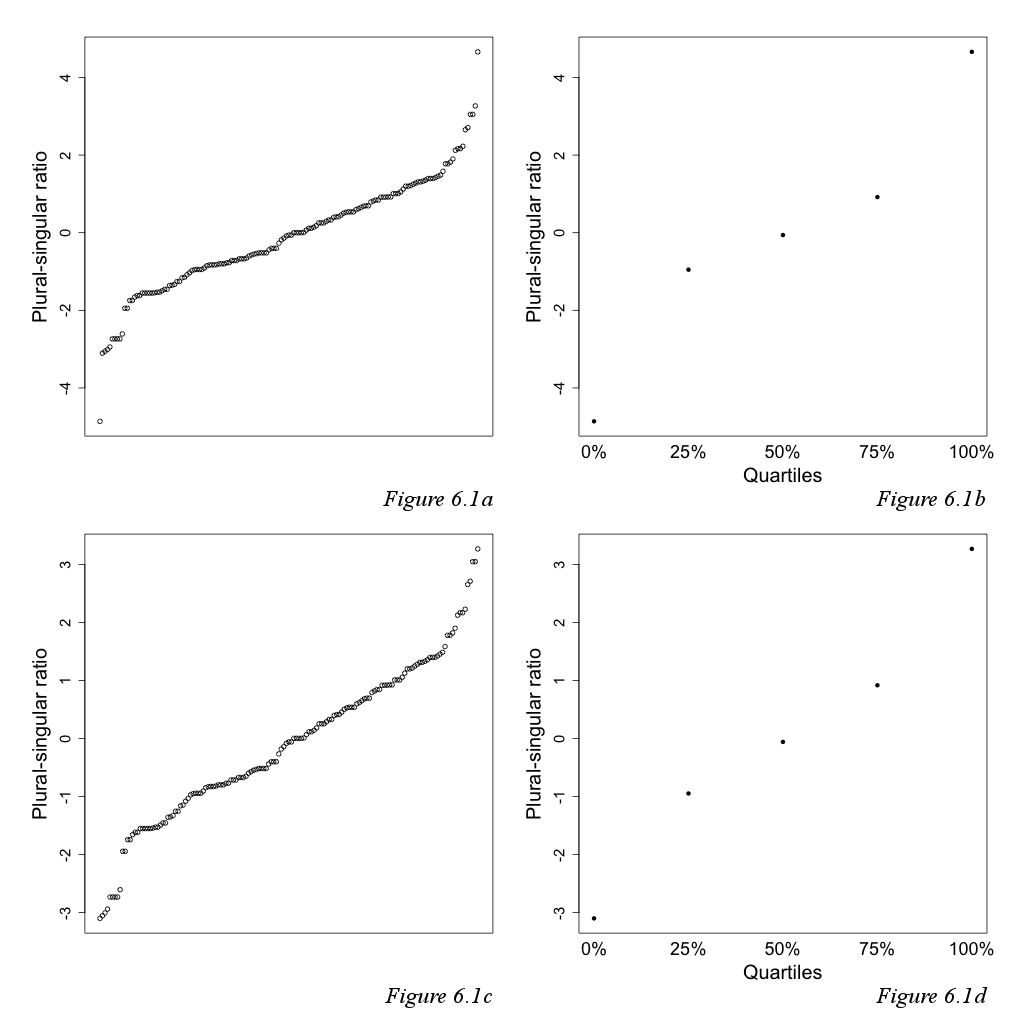
\includegraphics[width=\textwidth]{figures/6-Figure_1.png}
\caption{The ordered values of the plural-singular odds on the logarithmic scale (a) and its quartiles (b); before removing the outliers (c) and after removing outliers (d).\label{fig:6:1}}
\end{figure}

Figure \ref{fig:6:2} shows the relationship between the plural-singular ratio on the logarithmic scale and the language of the overt plural marker. The binary variable overt plural marker is on the vertical axis and has the values of one and zero, which represent the overt plural marker language, Russian, as the matrix language, and German, as the embedded language; the values of the odds are on the horizontal axis. The line depicting the relationship between the two variables is a LOWESS (locally weighted scatterplot smoothing) curve \citep{lowess}. As indicated in Figure \ref{fig:6:2}, the curve is virtually symmetrical around the logarithmic value of $-0.3$, which corresponds to the odds value of 0.740. In the plot we can also see that the line has two points of inflection, separating the central interval of the curve between the logarithmic values of $-1.3$ and 0.6. The central interval, also symmetrical around $-0.3$, stands for a gradual, transitional area. Interestingly, a comparison of the inflection points 0.277 and 1.822 at opposite ends of the spectrum also shows a symmetrical distribution of the lexical items in the data set: there are as many singular-dominant nouns as there are plural-dominant ones. As is evident from the shape of the curve, embedded-language nouns with embedded-language plural markers correspond to plural dominant nouns, whereas embedded-language nouns  featuring matrix language overt plural markers correspond to singular-dominant nouns. As such, the higher an embedded lexical item’s plural-singular ratio, or the odds, the more likely this item will appear with embedded-language plural marking in bilingual speech. Thus, embedded-language plurals appear to be accessed and selected in online speech production as units.

\begin{figure}
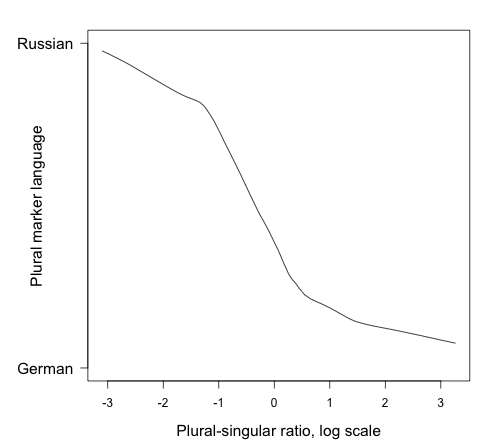
\includegraphics[scale=0.5]{figures/6-Figure_2.png}
\caption{The relationship between the plural-singular ratio (on the logarithmic scale) and the language of the overt plural marker. Russian is the matrix language (ML), German is the embedded language (EL).\label{fig:6:2}}
\end{figure}

\subsubsection{Stem-final segment of the insertion}

\noindent In this section I analyse the stem-final segment of an inserted lexical item as a predictor of the language of its plural marker. I identify stem-final segments of the nouns’ base forms, i.e., the forms in the nominative singular. For example, the stem-final segment of the word \textit{Türke} `Turk' is a vowel. As shown in \ref{morph-restr}, several strategies are employed to enable the addition of Russian inflectional suffixes, marking the plural, to German stems ending in vowels. As mentioned above, these strategies aim at hiatus resolution at the morpheme boundary. One strategy is to delete the vowel, if it is unaccented, regardless of its quality, as in (\ref{ex:6:19}), another option is to insert a consonant, or a consonant cluster, which, as a rule, correspond to parts of Russian derivational suffixes. Crucially, the need to resolve the morphophonological mismatch may also result in the use of German plural markers on German stems ending in vowels. This is particularly characteristic of stems whose final vowels are accented. In contrast to the morphophonological constraint formulated above, the assumption here is that even German nominal stems with unaccented vowels in the final position may tend to occur with German plural markers in otherwise Russian sentences. In other words, if the stem-final segment of the inserted lexical item is a vowel, the chance that this item will be used with a German plural marker is high, and vice versa, if the final segment of an inserted stem is a consonant, the preference for a Russian inflection in plural contexts will be strong.

The data were coded for the presence, or absence, of a vowel in the stem-final position of inserted German nouns. In the case of the stem-final /r/, its consonantal and vocal realisations were treated separately and were respectively coded. Figure \ref{fig:6:3} displays the relationship between the sound at the stem end and the language of the plural marker. According to Figure \ref{fig:6:3}, the proportion of embedded-language plural markers is skewed depending on whether stems feature final vowels. This is in line with the hypothesis that noun insertions with vowels in the stem-final position favour German plural markers, while Russian plural markers are more common on stems ending in consonants. Whether the segment in the stem-final position of a German insertion has explanatory power regarding the variation in the data will be further examined and discussed in \sectref{stat}.

\begin{figure}
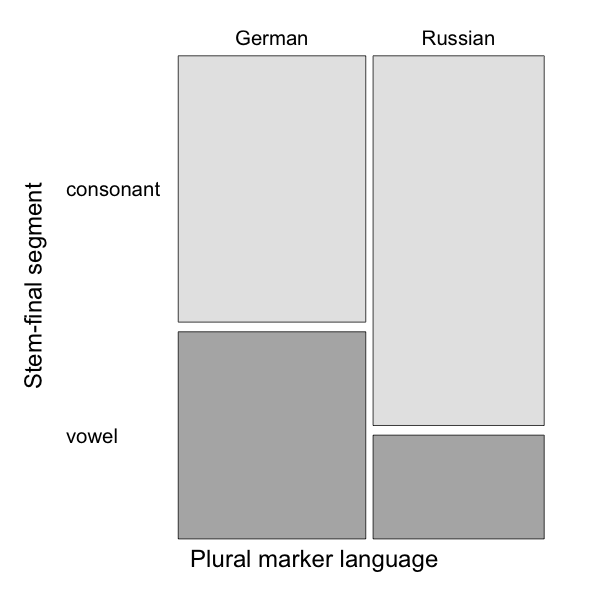
\includegraphics[scale=0.5]{figures/6-Figure_3.png}	
\caption{The relationship between the choice of the language for overt plural marking on German nominal insertions and the final sound of the stem. Russian is the matrix language (ML), German is the embedded language (EL).\label{fig:6:3}}
\end{figure}

\subsubsection{The morphological case of the slot}

The mismatch in the nominal systems of German and Russian could be considered an additional motivation to use Russian inflectional suffixes when inserting German lexical material into Russian sentences. The  languages are nonequivalent in two respects: First, the Russian morphological cases outnumber the German cases six to four. Second, case in German is principally not marked morphologically on the stem, but rather syntactically on the determiner (see \sectref{german}). However, my corpus contains no instances of insertion of fully-fledged noun phrases, nor is morphological marking by the dative suffix \textit{-(e)n} attested on inserted German plurals. Hence German plurals remain unmarked for the morphological case. In contrast, the degree of syncretism among Russian plural inflections is sizeably lower. In order to mark the case overtly and thus in line with the general pattern of the Russian nominal system, speakers may tend to utilise Russian plural markers, especially if the case projected on the slot is a non-core case, i.e., neither the nominative nor the accusative.


The nominative and the accusative case have a special status in the Russian declensional system. In the data set, the nominative plural is generally expressed by the inflection \textit{-i} and its phonological allomorph \textit{-y}, with the exception of the inflection of the masculine plural \textit{-á}, occurring in the form \textit{bauer-á} `peasants' in analogy with such Russian nouns as \textit{professor-á} and \textit{traktor-á}. The same inflections are used for the accusative plural of inanimate nouns. Note that no animate nouns are attested in the data set in the form of the accusative plural (which require inflections identical with the genitive plural). In other words, apart from one instance of the inflection \textit{-a}, the nominative plural and the accusative plural appear both to be marked solely by the inflection \textit{-i} and its allomorph \textit{-y}. As such, the inflection \textit{-i (-y)} is regarded as a prototypical plural marker of Russian nouns; the inflection \textit{-y} also marks plural on predicative short adjectives, as in \textit{umn-y} `clever-\textsc{pl}', and the inflection \textit{-i} marks the plural on verbs in the past tense, as in \textit{by-l-i} `be-\textsc{past-pl}', thus reinforcing their status as prototypical plural markers. Additional evidence for this assumption comes from language acquisition. As the most frequent plural inflection in the declensional system of Russian nouns, \textit{-i (y)} is the first plural inflection to be acquired by Russian learning children and is the one most often generalised in the process of acquisition \citep{gagarina-voeikova}. As previously outlined, the status of this formative is similar to the status of German plural inflections in that they are also distinguished by syncretism. We may assume that similarity between German plural markers and Russian inflections expressing the plural in the core cases facilitates insertion of German plural forms. In other words, if the case projected on the slot is nominative or accusative, German plurals can be accommodated easily. The opposite seems to hold as well: German noun stems will take Russian plural inflections if the slots in which they are inserted require non-core cases.

These hypotheses determined the coding of the data with respect to the case. The German noun insertions examined were analysed for the morphological case projected on the slot in which they were inserted. Following the argumentation above, the items fell into two groups: one group included the items in nominative and accusative slots, and the other group was made up of the items in the non-core cases, namely, the genitive, the dative, the instrumental and the prepositional. Thus, the predictor “case of the slot” was handled as a binary variable. The relationship between the case projected on German noun insertions and the language of the plural marker is displayed in \ref{fig:6:4}. The case of the slot is on the vertical axis, the language of the plural marker is on the horizontal axis. The data in \ref{fig:6:4} reveal that overall, the nominative and the accusative are more frequent than all the other cases. Additionally, the proportions of the embedded-language plural markers and the matrix language plural markers are asymmetrical in terms of the case required by the slot. The large proportion of German plurals in the nominative and accusative slots indicates that these slots, as expected, favour the insertion of German plurals. I interpret this fact by similarity in the status between the Russian inflectional suffix(es) of the nominative/accusative plural and German plural markers. Their status is similar because like German plural markers, which express the number, the Russian plural suffix \textit{-i} (\textit{-y}) also expresses the number in the first place, blurring the distinction between the nominative and the accusative. Finally, as anticipated, inflections of the matrix language are preferred when a non-core case is required. Given these considerations, the case projected on the slot will be included in the multi-factorial statistical analysis below as a factor determining the language of the plural marker.

\begin{figure}
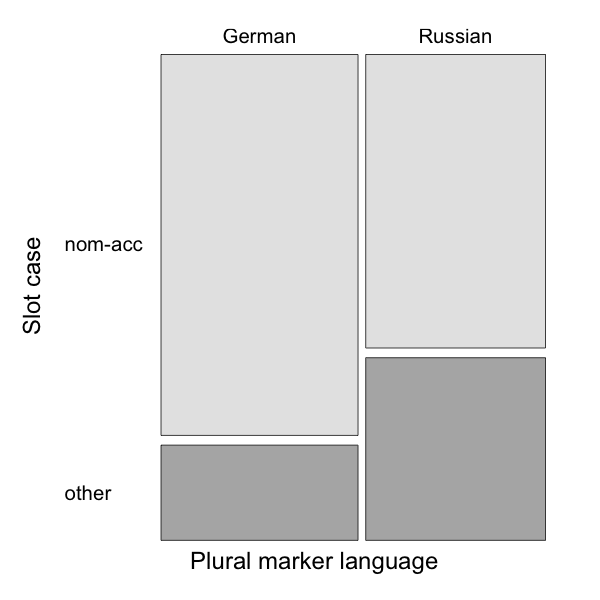
\includegraphics[scale=0.5]{figures/6-Figure_4.png}
\caption{The relationship between the choice of the language for overt plural marking on German (EL) nominal insertions and the case projected by the slot. Russian is the matrix language (ML).\label{fig:6:4}}
\end{figure}

\section{Statistical model}\label{stat}

In this section, I will investigate the factors presented thus far with regard to the extent to which they compete with, or assist, one another in determining the plural marking on German nouns inserted into a Russian matrix structure. I will also examine and assess each of the competing factors’ explanatory power. To approach these issues, I will adopt the procedure employed in the foregoing chapters, which included the fitting and evaluation of a generalised linear mixed model (see \citealt[278--284]{baayen-analyzing}). In this model, significant interactions between the predictor variables outlined above and the binary dependent variable “the language of the plural marker on code-mixed German nouns” will provide tangible evidence for the relevance of the predictor variables.

\subsection{Model fitting}

In order to obtain a minimal adequate regression model, the common procedure was employed \citep{baayen-analyzing,szmrecsanyi-2013}, which included fitting the maximal model with the three factors outlined above as main effects: the odds, based on the distribution frequencies of the inserted noun's singulars and plurals in the embedded language; this item’s stem-final segment, i.e., a vowel or a consonant; and the morphological case of the slot in which the item is inserted. Additionally, the maximal model included the interactions between these factors. The speakers' individual differences in marking plural on German nominal insertions, i.e., the tendency to either retain the German plural marker or to add Russian plural inflections, was measured by means of the variable “speaker”. The variable “speaker” was handled as a by-subject random effect. Unfortunately, adding “item” as a random effect was impossible due to the high variation in this variable: 151 German noun insertions correspond to 110 different lexical items. The model was thus run without the by-item variable. The model simplification consisted in the exclusion of factors and interactions without any significant contribution to the explanatory power of the model. Following \citet[281]{baayen-analyzing}, the estimation of explanatory power of the interaction terms and main effects is based on the calculation of the \textit{C} index of concordance. In line with the reduction procedure, all interaction terms were excluded from the model (plural-singular ratio $\times$ stem-final segment, plural-singular odds ratio $\times$ case of the slot, stem-final segment $\times$ case of the slot). The final, minimal adequate model is given in Table \ref{tab:6:6}.

\begin{table}
		\begin{tabular}{l rrr l}
		 \lsptoprule
	     Factor & Odds & Est. & $\text{Pr}(>|z|)$ & \\\midrule
		(Intercept) & 2.147 & 0.764  & 0.096 & \\
			Plural-singular ratio & 0.443 & −0.815 & 0.000 & ***\\
			Stem-final segment (`vowel') & 0.339 & −1.082 & 0.014 & *\\ 
			Slot case (`\textsc{nom} or \textsc{acc}') & 0.383 & −0.961 & 0.031 & *\\\midrule
			\multicolumn{5}{l}{Random effect:}\\
			\multicolumn{5}{l}{Speaker}\\
			\multicolumn{5}{l}{(intercept, $N = 12, \text{variance} = 0.439, \sigma = 0.662$)}\\\midrule
			\multicolumn{2}{l}{Summary statistics:}\\
			\multicolumn{2}{l}{$N$} & 151 &\\
			\multicolumn{2}{l}{\% correct predictions (\% baseline)} & 79 (81) &\\
			\multicolumn{2}{l}{\textit{C} index of concordance} & 0.838 & \\
			\multicolumn{2}{l}{Somer's Dxy}  & 0.676 & \\
			\lspbottomrule
		\end{tabular}
	\caption{Predicting the language of the overt plural marker: minimal adequate generalized linear mixed model. Predicted odds ratios are for Russian (or matrix language) overt plural markers. Significance codes: *significant at $p < 0.05$, ** $p < 0.01$, *** $p < 0.001$.}
\label{tab:6:6}
\end{table}

\subsection{Model evaluation and model discussion}

After the model is fit to the data, the fit can be evaluated. The minimal adequate model reported in Table \ref{tab:6:6} is of high quality. The model correctly classifies 79\% of the data overall. Regarding the categorical prediction of the plural marker language, i.e., when always guessing one variant, the model correctly predicts 77\% of German plural markers and 81\% of Russian plural inflections. Furthermore, the fit is estimated by the measure of predictive accuracy which relates the observed realisations of the plural marker to the predicted outcome of the model \citep{bresnan-etal}. The outcome of the model is the choice of the German or Russian plural marker, denoted by 0 and 1 respectively. The accuracy measure counts any probability >{} 0.5 as correct for the Russian plural marker. The measure of predictive accuracy is provided in Table \ref{tab:6:7}. The model correctly predicts the use of German plural markers with the lexical items analysed in 85\% of the cases, but it has more difficulty predicting the use of Russian plural markers, performing with only 72\% of correct predictions. The \textit{C} index of concordance between the predicted probability and the observed binary outcome is 0.838, which indicates that the model has real predictive power. Performance indicator Somers' Dxy, a rank correlation coefficient between predicted probabilities and observed binary response, is 0.676, which also attests some predictive capacity of the model. As to the random effect “speaker”, the variance and standard deviation of the by-subject effect reveal minimal variation. The speakers in the sample favour neither language for marking the plural on German insertions at the individual level.

\begin{table}
		\begin{tabular}{l cccc} 
		\lsptoprule
 			&& \multicolumn{2}{c}{Predicted} &\% correct\\\cmidrule(lr){3-4}
			  & &0 &1 &\\ \midrule
			Observed  & 0     &67   &12 &85\\
			 &1 &20 &52 &72\\
			 Overall & & & &79\\
			 \lspbottomrule
		 \end{tabular}
		 \caption{Model accuracy. Classification table for the minimal adequate model. (The table representation is based on \citealt{bresnan-etal}).\label{tab:6:7}}
\end{table}

The main effects in the model offer persuasive evidence in favour of the hypotheses formulated above. The signs of the regression coefficients (Estimate) in Table \ref{tab:6:6} reveal the direction of the adjustment to the intercept. Given this, we can conclude that the factors a noun’s plural dominance, or high plural-singular ratio, vowel as the final segment of the stem, and the nominative or accusative case of the slot disfavour the use of Russian plural markers with German code-mixed nouns. Conversely, any of the non-core cases projected on the slot, a consonant as the final segment of the stem, and a noun's singular dominance, or low plural-singular ratio, demonstrate a preference for Russian plural markers. Consider the odds listed in Table \ref{tab:6:6}. Both the stem-final segment and the case of the slot have comparable effect sizes, that is, the odds for using a Russian plural marker decrease by approximately 66\% if the stem features a vowel in the final position, and by 62\% if the case of the slot is either nominative, or accusative. The strongest effect is exerted by the plural-singular ratio, or dominance: the odds for Russian overt plural markers fall by 56\% at every one-unit increase in the plural-singular ratio on the logarithmic scale. This stands for the increase of this ratio by 2.7 on the linear scale. In other words, if the plural-singular ratio increases by 2.7, the odds for using a Russian plural marker falls by 56\%. The overall importance of the factors is given in Figure \ref{fig:6:5} by plotting the decreases in the Akaike Information Criterion of the model when a factor is removed from the minimal model. As mentioned in the previous chapters, more sizable decreases in the AIC criterion of a factor stand for its greater overall importance. Thereby, when predicting the language of the overt plural marker used with 151 German noun insertions in Russian sentences, the most important factor is the plural-singular ratio. The second most important predictor is the phonemic shape of the stem, namely, the presence or absence of a vowel in the stem-final position. The case projected by the slot on the inserted lexical item is ranked last. Crucially, in slots projecting the nominative or the accusative case (coded as one level of the binary variable “case of the slot”) the proportions of German and Russian plural markers on noun insertions are equally large, and the asymmetry exhibited is due to the number of instances of the other cases projected. In this case, German noun insertions do not take German plural markers as frequently as Russian ones.

\begin{figure}
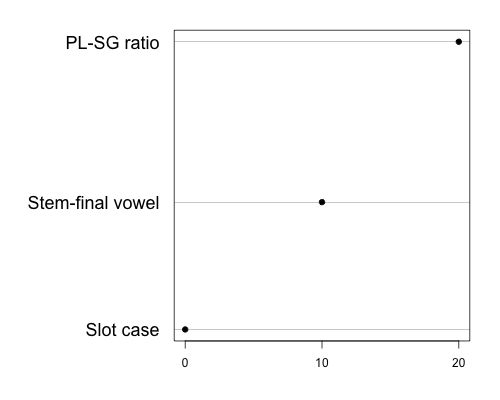
\includegraphics[scale=0.5]{figures/6-Figure_5.png}
\caption{Importance of factors in model: decrease in Akaike Information Criteri-on (AIC) if factor removed. (The table representation is based on \citealt{szmrecsanyi-2013}).\label{fig:6:5}}
\end{figure}

This analysis shows that the frequency-based plural-singular ratio, a continuous variable, and structural factors such as the case of the slot and the the inserted lexical item’s stem-final segment  reliably predict the language of the overt plural marker on German lexical items inserted in Russian matrix frames, the most important predictor of this variation being the plural-singular ratio. The variation in the speakers' preferences to use either Russian or German plural markers was taken into consideration and found to be negligible.

\section{Conclusions and discussion}

%In an attempt to predict this variation, the current study draws on assumptions stemming from usage-based approaches. A usage-based approach not only aims to provide a cognitively real account of language processing and organization, it also allows for an integration of two kinds of factors: factors based on discreet categories, and factors distinguished by gradience. In order to test the interplay of these probabilistic factors and predict its outcome, a statistical model is applied.

\noindent This study has addressed the question of whether in a situation of marking plural on code-mixed lone nouns, these nouns retain the plural morphology of their language, i.e., the embedded language, or receive plural markers from the matrix language: {\textsubscript{R}[ \textsubscript{G}[~N \textsubscript{G}]-\textsc{pl} \textsubscript{R}]} or {\textsubscript{R}[ \textsubscript{G}[ N-\textsc{pl} \textsubscript{G}] \textsubscript{R}]}. Prior research has largely focused on explaining the use of either double plural morphology or embedded-language plural morphology with code-mixed nouns, and attributed the use of these patterns to structural factors (\citealt[91]{boumans-syntax-1998}; \citealt[91]{myers-scotton-contact-2002}, 150), erroneous access in production (\citealt[132--136]{myers-scotton-duelling-1993}; \citealt[1000]{myers-scotton-matching-1995}) or high frequency of some plurals in the source language (\citealt[151]{backus-two-1996}, \citeyear[97--99]{backus-evidence-1999}, \citeyear[93--100]{backus-units-2003}). However, these assumptions have neither been systematically examined, nor tested on monolingual material. In this study I have analysed the extent to which the choice of the language of plural marking on code-mixed nouns is determined by the frequency distribution of the inserted items’ singulars and plurals in the embedded language and the structural requirements imposed by the matrix language. The research questions are addressed through corpus analyses and statistical modelling.

This investigation reveals three main findings. The first concerns a frequency effect: the frequency with which a noun’s plural occurs in the embedded language, i.e., German, appears to determine the language of the plural marker on code-mixed nouns. In a situation of competition between a lexeme’s singular and plural forms during online production, a plural-dominant item tends to be selected as a whole and inserted into a matrix clause together with its plural marker. If the inserted lexical item is a singular-dominant noun, only the stem, which corresponds to the base form in these data, will be activated in production and will receive the plural marker from the matrix language, namely, Russian. This provides compelling evidence for the effect of frequency assumed earlier in \citep{backus-two-1996,backus-evidence-1999, backus-units-2003}.

The entrenchment of high-frequency plurals observed in the Russian-German code-mixing data concurs with similar findings from previous studies in language processing, first-language acquisition and typology. Experimental research into processing of singulars and plurals has produced substantial evidence that plural-dominant words are accessed faster than singular-dominant words \citep{new-etal-2004,sereno-jongman-1997,baayen-dijkstra-schreuder}. This frequency effect is interpreted as evidence for the fact that a plural-dominant word is accessed directly and has an allocated autonomous representation in the mental lexicon. In the speech of children acquiring Russian, the first plural forms are nouns that are usually used as plurals, for example, \textit{glaz-a} `eye-\textsc{nom.pl}', \textit{jagod-y} `berry-\textsc{nom.pl}' and \textit{grib-y} `mushroom-\textsc{nom.pl}' \citep[198]{gagarina-voeikova}. Interestingly, children have been found to use these forms with reference to singular entities \citep[91]{ceitlin}, which reinforces the idea that plural-dominant nouns are learned and retrieved as holistic units. Furthermore, in a corpus-based cross-linguistic study of number marking, \citet{haspelmath-karjus} propose semantic groups of lexemes which are more frequent as plurals than singulars, these include paired body-parts, paired items, small animals, fruit/vegetables, people, and ethnic groups. It is indeed striking that many of the insertions with the embedded-language plural markers in both my data and other bilingual corpora fall into one of the suggested categories. The frequency effect observed in my data might also be approached from a semantic perspective.

The second finding of this study concerns the relevance of the phonemic shape of the inserted word to the likelihood of receiving an inflectional suffix from the matrix language. I have shown that a German lexical item with an accented vowel in the stem-final position cannot take Russian inflectional suffixes directly since the Russian declensional system depends on stems with consonants in the final position. If the final segment of an inserted German stem is an accented vowel, either a compromise strategy such as the use of epenthetic consonants is employed, or German plural forms are produced. Therefore, the Russian declensional system restricts the use of Russian inflectional suffixes with German stems depending on their phonemic shapes. In the subsequent statistical model, I reconsidered this absolute constraint as a probabilistic factor because the across-the-board analysis revealed that the presence of a vowel in the stem-final position, whether accented or not, results in favouring the use of German plural markers. This effect is grounded in processes of similarity identification between Russian inflected words and German insertions at the level of morphophonology. Instances of accommodation of German nouns when bilingual speakers reanalyse some of the stems' material as part of Russian derivational suffixes demonstrate that when similarity between German and Russian forms is lacking, speakers construct similarity online \citep[cf.][]{hakimov-backus-20-intro}, in order to produce forms satisfying the requirements of the matrix language and being thus acceptable in the bilingual community. 

The third result relates to the other structural factor: the mismatch in the systems of case marking in the plural between German and Russian. When the matrix structure projects a non-core case on the slot in which a German lexical item is inserted, the tendency is to employ Russian inflections, characterised by a fusion of the number and the case. This finding can be interpreted as a manifestation of the pressure exerted by the matrix language to produce well-formed Russian constituents. Nonetheless, many German plural nouns occur in slots requiring the nominative or accusative case. This situation is explained by the fact that the functions of German plural inflections and the Russian inflection of the nominative and accusative case \textit{-i (y)} coincide: owing to form syncretism, both express the plural number rather than the case. This kind of equivalence results in the ease of inserting German plurals in such slots. We may also assume that the declensional systems of the two languages are perceived as incompatible in the other morphological cases because in slots projecting these cases, bilingual speakers tend to use Russian (=matrix language) plural formatives, enabling unambiguous case-marking.

The findings of this study have far-reaching consequences for models of code-mixing because they clarify the emergence of the so-called internal embedded-language islands. Firstly, the embedded-language plural markers are regarded as syntactically inactive \citep[92]{myers-scotton-contact-2002} or parts of chunks \citep[98]{backus-evidence-1999}. If we combine the concept of syntactic inactivity with the idea of holistic storage, we can assert that embedded-language plural markers are syntactically inactive inasmuch as they are part of the representations of plural forms. These plurals are so strongly entrenched in the mental lexicon/grammar that they are retrieved as wholes in bilingual production. If a plural is weakly entrenched, a matrix language plural marker is produced. Secondly, by handling both categorical variables -- the phonetic and the morphosyntactic context -- as probabilistic tendencies rather than absolute constraints, the study has provided greater understanding of non-trivial idiosyncrasies observed in bilingual language production. Thirdly, the findings demonstrate that in language mixing at the level of morphology, bilingual speakers keep track of the regularities and distribution properties of both the embedded language and the matrix language. While the matrix language determines the morphosyntactic and phonetic context and thus influences the choice between the competing mixing patterns, the distribution properties of the embedded-language material appears to play even a greater role in predicting the examined variation. Similarity identification, which manifests itself at the level of morphophonology and the level of morphosyntax, again involves activation of the representations attributed to both languages. The results reported here are encouraging, and should be validated in further studies of other bilingual corpora.

The study presented in this chapter differs from the studies reported in the previous chapters in that it showcases how frequency-based and structural factors can be usefully investigated together as factors influencing choices between variant mixing patterns in bilingual speech. I have interpreted the effects of contextual structural factors within the framework of usage-based contact linguistics, arguing that processes of similarity detection, and even construction, are at the core of the choices which bilingual speakers make in online speech production.
